%%%%%%%%%%%%%%%%%%%%%%%%%%%%%%%%%%%%%%%%%%%%%%%%%%%%%%%%%%%%%%%%%%%%%%%
%DIF LATEXDIFF DIFFERENCE FILE
%DIF DEL DMCfun.tex        Sat Apr  4 10:52:10 2020
%DIF ADD DMCfun_rev1.tex   Sat Apr  4 12:43:11 2020
%                       Springer Latex Template                       %
%%%%%%%%%%%%%%%%%%%%%%%%%%%%%%%%%%%%%%%%%%%%%%%%%%%%%%%%%%%%%%%%%%%%%%%

%%%%%%%%%%%%%%%%%%%%%%%%%%%%%%%%%%%%%%%%%%%%%%%%%%%%%%%%%%%%%%%%%%%%%%%
%                              EPS File                               %
%%%%%%%%%%%%%%%%%%%%%%%%%%%%%%%%%%%%%%%%%%%%%%%%%%%%%%%%%%%%%%%%%%%%%%%
% First comes an example EPS file -- just ignore it and
% proceed on the \documentclass line
% your LaTeX will extract the file if required
\begin{filecontents*}{example.eps}
%!PS-Adobe-3.0 EPSF-3.0
%%BoundingBox: 19 19 221 221
%%CreationDate: Mon Sep 29 1997
%%Creator: programmed by hand (JK)
%%EndComments
gsave
newpath
  20 20 moveto
  20 220 lineto
  220 220 lineto
  220 20 lineto
closepath
2 setlinewidth
gsave
  .4 setgray fill
grestore
stroke
grestore
\end{filecontents*}
\RequirePackage{fix-cm}



%%%%%%%%%%%%%%%%%%%%%%%%%%%%%%%%%%%%%%%%%%%%%%%%%%%%%%%%%%%%%%%%%%%%%%%
%                           Start Document                            %
%%%%%%%%%%%%%%%%%%%%%%%%%%%%%%%%%%%%%%%%%%%%%%%%%%%%%%%%%%%%%%%%%%%%%%%
\documentclass[]{svjour3}\usepackage[]{graphicx}\usepackage[]{color}
% maxwidth is the original width if it is less than linewidth
% otherwise use linewidth (to make sure the graphics do not exceed the margin)
\makeatletter
\def\maxwidth{ %
  \ifdim\Gin@nat@width>\linewidth
    \linewidth
  \else
    \Gin@nat@width
  \fi
}
\makeatother

\definecolor{fgcolor}{rgb}{0.345, 0.345, 0.345}
\newcommand{\hlnum}[1]{\textcolor[rgb]{0.686,0.059,0.569}{#1}}%
\newcommand{\hlstr}[1]{\textcolor[rgb]{0.192,0.494,0.8}{#1}}%
\newcommand{\hlcom}[1]{\textcolor[rgb]{0.678,0.584,0.686}{\textit{#1}}}%
\newcommand{\hlopt}[1]{\textcolor[rgb]{0,0,0}{#1}}%
\newcommand{\hlstd}[1]{\textcolor[rgb]{0.345,0.345,0.345}{#1}}%
\newcommand{\hlkwa}[1]{\textcolor[rgb]{0.161,0.373,0.58}{\textbf{#1}}}%
\newcommand{\hlkwb}[1]{\textcolor[rgb]{0.69,0.353,0.396}{#1}}%
\newcommand{\hlkwc}[1]{\textcolor[rgb]{0.333,0.667,0.333}{#1}}%
\newcommand{\hlkwd}[1]{\textcolor[rgb]{0.737,0.353,0.396}{\textbf{#1}}}%
\let\hlipl\hlkwb

\usepackage{framed}
\makeatletter
\newenvironment{kframe}{%
 \def\at@end@of@kframe{}%
 \ifinner\ifhmode%
  \def\at@end@of@kframe{\end{minipage}}%
  \begin{minipage}{\columnwidth}%
 \fi\fi%
 \def\FrameCommand##1{\hskip\@totalleftmargin \hskip-\fboxsep
 \colorbox{shadecolor}{##1}\hskip-\fboxsep
     % There is no \\@totalrightmargin, so:
     \hskip-\linewidth \hskip-\@totalleftmargin \hskip\columnwidth}%
 \MakeFramed {\advance\hsize-\width
   \@totalleftmargin\z@ \linewidth\hsize
   \@setminipage}}%
 {\par\unskip\endMakeFramed%
 \at@end@of@kframe}
\makeatother

\definecolor{shadecolor}{rgb}{.97, .97, .97}
\definecolor{messagecolor}{rgb}{0, 0, 0}
\definecolor{warningcolor}{rgb}{1, 0, 1}
\definecolor{errorcolor}{rgb}{1, 0, 0}
\newenvironment{knitrout}{}{} % an empty environment to be redefined in TeX

\usepackage{alltt}  % [] or [smallcondensed], [smallextended], [twocolumn]

\usepackage{tempora}  % use Times fonts if available on your TeX system
\usepackage{graphicx}
\usepackage{color}
\usepackage{float}
\usepackage{listings}
\usepackage{longtable}
\usepackage[style=apa, sortcites=true, sorting=nyt,backend=biber]{biblatex}

\addbibresource{bibfile.bib}

% R syntax colours
\definecolor{dkgreen}{rgb}{0,0.6,0}
\definecolor{blue}{rgb}{0.0,0.0,1.0}
\definecolor{black}{rgb}{0.0,0.0,0.0}
\definecolor{white}{rgb}{1.0, 1.0, 1.0}

% % https://tex.stackexchange.com/questions/132582/transparent-foreground-watermark
% \usepackage{tikz}
% \usepackage[printwatermark]{xwatermark}
% \newsavebox\mybox
%DIF 110a110
 %DIF > 
%DIF -------
% \savebox\mybox{\tikz[color=gray, opacity=0.5]\node{DRAFT};}
% \newwatermark*[ allpages, angle=45, scale=10, xpos=-50, ypos=50 ]{\usebox\mybox}

\lstdefinestyle{R}
{
  language=R,
  basicstyle=\small\ttfamily,
  backgroundcolor=\color{white},
  frame=single,
  rulecolor=\color{black},
  tabsize=4,
  columns=fullflexible,
  keepspaces=true,
  breaklines=true,
  breakatwhitespace=false,
  keywordstyle=\color{black},
  commentstyle=\color{dkgreen},
  stringstyle=\color{black}
}

\journalname{Behavior Research Methods}
\IfFileExists{upquote.sty}{\usepackage{upquote}}{}
%DIF PREAMBLE EXTENSION ADDED BY LATEXDIFF
%DIF UNDERLINE PREAMBLE %DIF PREAMBLE
\RequirePackage[normalem]{ulem} %DIF PREAMBLE
\RequirePackage{color}\definecolor{RED}{rgb}{1,0,0}\definecolor{BLUE}{rgb}{0,0,1} %DIF PREAMBLE
\providecommand{\DIFadd}[1]{{\protect\color{blue}\uwave{#1}}} %DIF PREAMBLE
\providecommand{\DIFdel}[1]{{\protect\color{red}\sout{#1}}}                      %DIF PREAMBLE
%DIF SAFE PREAMBLE %DIF PREAMBLE
\providecommand{\DIFaddbegin}{} %DIF PREAMBLE
\providecommand{\DIFaddend}{} %DIF PREAMBLE
\providecommand{\DIFdelbegin}{} %DIF PREAMBLE
\providecommand{\DIFdelend}{} %DIF PREAMBLE
\providecommand{\DIFmodbegin}{} %DIF PREAMBLE
\providecommand{\DIFmodend}{} %DIF PREAMBLE
%DIF FLOATSAFE PREAMBLE %DIF PREAMBLE
\providecommand{\DIFaddFL}[1]{\DIFadd{#1}} %DIF PREAMBLE
\providecommand{\DIFdelFL}[1]{\DIFdel{#1}} %DIF PREAMBLE
\providecommand{\DIFaddbeginFL}{} %DIF PREAMBLE
\providecommand{\DIFaddendFL}{} %DIF PREAMBLE
\providecommand{\DIFdelbeginFL}{} %DIF PREAMBLE
\providecommand{\DIFdelendFL}{} %DIF PREAMBLE
%DIF LISTINGS PREAMBLE %DIF PREAMBLE
\RequirePackage{listings} %DIF PREAMBLE
\RequirePackage{color} %DIF PREAMBLE
\lstdefinelanguage{DIFcode}{ %DIF PREAMBLE
%DIF DIFCODE_UNDERLINE %DIF PREAMBLE
  moredelim=[il][\color{red}\sout]{\%DIF\ <\ }, %DIF PREAMBLE
  moredelim=[il][\color{blue}\uwave]{\%DIF\ >\ } %DIF PREAMBLE
} %DIF PREAMBLE
\lstdefinestyle{DIFverbatimstyle}{ %DIF PREAMBLE
	language=DIFcode, %DIF PREAMBLE
	basicstyle=\ttfamily, %DIF PREAMBLE
	columns=fullflexible, %DIF PREAMBLE
	keepspaces=true %DIF PREAMBLE
} %DIF PREAMBLE
\lstnewenvironment{DIFverbatim}{\lstset{style=DIFverbatimstyle}}{} %DIF PREAMBLE
\lstnewenvironment{DIFverbatim*}{\lstset{style=DIFverbatimstyle,showspaces=true}}{} %DIF PREAMBLE
%DIF END PREAMBLE EXTENSION ADDED BY LATEXDIFF

\begin{document}
\title{DMCfun: An R package for fitting Diffusion Model of Conflict (DMC) to reaction time and error rate data}
\subtitle{}
\titlerunning{DMCfun}

\author{Ian G. Mackenzie \and
    Carolin Dudschig
}

\institute{Ian G. Mackenzie \at
    Schleichstrasse 4, Rm 4.427\\
    Tübingen\\
    Germany\\
    Tel.: +49 (0)7071 29-75589\\
    \email{ian.mackenzie@uni-tuebingen.de}
}

\date{Received: date / Accepted: date}
\maketitle

\begin{abstract}

    Decision processes within choice reaction-time (CRT) tasks are often
    modelled using variations of a Diffusion Decision Model \DIFdelbegin \DIFdel{(DDM, for a review, see
    \textcite{ratcliff2008diffusion})}\DIFdelend \DIFaddbegin \parencite[DDM, for
    a review, see][] {ratcliff2008diffusion}\DIFaddend . \textcite{ulrich2015automatic}
    introduced a Diffusion Model for Conflict tasks (DMC). The DMC model
    combines common features from within standard diffusion models with the
    addition of superimposed controlled and automatic activation. The DMC model
    is used to explain distributional reaction time (and error rate) patterns
    in common behavioural conflict-like tasks (e.g., Flanker task, Simon task).
    This paper introduces the R-package DMCfun, which implements the DMC model
    and provides functionality to fit the model to observed data.

\keywords{reaction time \and conflict task \and Diffusion Model Conflict (DMC) \and R package}

\end{abstract}

\section{Introduction}
\label{introduction}

Conflict tasks \DIFdelbegin %DIFDELCMD < \parencite[e.g., Flanker task, Simon task, Stroop task,
%DIFDELCMD < see][]{eriksen1974effects, lu1995influence, macleod1991half}%%%
\DIFdel{, respectively) }\DIFdelend \DIFaddbegin \parencite[e.g., Flanker task, Simon task, Stroop task,
see][, respectively]{eriksen1974effects, lu1995influence, macleod1991half} \DIFaddend are
common experimental paradigms used to investigate decision processes under
response competition (i.e., the activation of competing response alternatives).
Such conflict tasks involve stimuli with multiple features that are either
relevant or irrelevant to the required task. For example, a typical Flanker
task consists of an array (e.g., HHHHH, HHSHH) with the central item being the
``target'' (task-relevant) and the surrounding items being the
``flankers'' (task-irrelevant). Responses are typically mapped to the left and
right hand (e.g., H = left, S = right). When the target and the flankers match
(mismatch), both the relevant and irrelevant dimensions indicate the same
(different) response. In a typical Simon task, participants respond to a
feature of a stimulus (e.g., colour, shape; relevant dimension) that is
presented at different spatial locations (e.g., left vs. right side of the
screen; irrelevant dimension). Again, responses are mapped to the left and
right hands (e.g., blue = left, red = right). When a stimulus presented in a
left (right) location requires a left-hand response, the relevant and
irrelevant stimulus dimensions match (mismatch). In such tasks, responses are
typically faster and less error-prone when the relevant and irrelevant response
dimensions indicate the same response (compatible) than when they indicate
different responses (incompatible). The longer reaction time and larger error
rate in incompatible trials indicates that task-irrelevant information
interferes with the processing of the task relevant information.

This compatibility effect pattern is consistent across all conflict-like tasks.
However, when the size of the effect (incompatible - compatible) is compared
across different percentiles of the RT distribution, different patterns can
emerge. Such differences across the RT distribution are investigated via the
use of delta functions (or delta plots) \parencite{de1994conditional,
speckman2008delta}. Such plots depict the compatibility effect (y-axis) at n
bins (x-axis) (see Figure \ref{fig:1} bottom-right panel for an example of a
delta plot). Such distributional analyses have indicated that the compatibility
effect in some conflict tasks (e.g., Stroop task) increases with slower
responses (i.e., positive-going delta slope) whereas in other conflict tasks
(e.g., Simon task) smaller compatibility effects are observed with slower
responses (i.e., negative-going delta slope) \parencite[see][for Stroop and
Simon tasks]{pratte2010exploring}.

The observation of both positive and negative-going delta slopes across
different conflict tasks has strong theoretical implications for processing
models of RT. For example, traditional diffusion models of RT cannot account
for negative-going delta functions \parencite{pratte2010exploring}. These
models propose that task-relevant information accumulates over time until one
of two decision boundaries is reached (correct vs. incorrect response
boundary). \textcite{wagenmakers2007linear} demonstrate that the positive
relationship between the mean and standard deviation of RT excludes the
possibility of observing negative-going delta functions. As summarized by
\textcite{ulrich2015automatic}, traditional RT models have difficulty
explaining negative-going delta functions. The DMC model is an extension of the
standard diffusion model that can explain observed delta functions (both
positive and negative going) across a range of conflict tasks. Since its
publication, simulation and fitting procedures of the DMC model have been
applied in various research \DIFdelbegin \DIFdel{context }\DIFdelend \DIFaddbegin \DIFadd{contexts }\DIFaddend in order to provide important insights into
the mechanisms at play in conflict tasks\parencite[e.g.,][]{servant2016,
mittelstadt2020beyond}.

Conditional accuracy functions (CAFs) also offer an additional tool with which
to investigate compatibility effects across the RT distribution. Here, accuracy
rates are calculated across N equally sized RT bins. For compatible trials,
accuracy is typically high across all bins, whereas for incompatible trials,
the lowest level of accuracy is observed at fastest RT bins. At the slowest RT
bins, there is little difference in accuracy between compatible and
incompatible conditions.

The following section introduces the DMC model \textcite{ulrich2015automatic}.
It must be noted that other extensions of standard drift diffusion models with
specific reference to conflict-like tasks have been proposed. For example, the
dual-stage two-phase model \DIFdelbegin \DIFdel{(DSTP; \textcite{hubner2010dua}) }\DIFdelend \DIFaddbegin \parencite[DSTP, ][]{hubner2010dual} \DIFaddend or the shrinking
spotlight model \DIFdelbegin \DIFdel{(SSP; \textcite{white2011diffusio})}\DIFdelend \DIFaddbegin \parencite[SSP, ][]{white2011diffusion}\DIFaddend . A direct comparison
between such models is beyond the scope of the current paper with such
comparisons provided elsewhere \parencite[see][albeit with specific reference
to the flanker task only]{white2018testing, evans2020comparison}.

\subsection{DMC Model Details} 
\label{model_details} 

The DMC model of \textcite{ulrich2015automatic} builds upon the idea that
conflict tasks consist of two processes that proceed in parallel (automatic and
controlled processing). Here, controlled processing concerns the task-relative
information, whereas automatic processing concerns the task-irrelevant
information. Whilst the architecture of such combined controlled/automatic
processing within individual conflict tasks is under-specified,
\textcite{ulrich2015automatic} suggest two possible architectures
\DIFdelbegin %DIFDELCMD < \parencite[see Figure 1][]{ulrich2015automatic} %%%
\DIFdelend \DIFaddbegin \parencite[see Figure 1 in ][]{ulrich2015automatic} \DIFaddend under which automatic and
controlled processing interact. Under both architectures, DMC assumes that a
single accumulation process (combined automatic and controlled) determines the
executed response. Critically, automatic processes will facilitate (impede)
controlled processes in compatible (incompatible) trials. In addition, it is
assumed that the activation output from automatic processes increases to a
maximum before decreasing back to zero (pulse function).

The formal model specification for DMC is provided in
\textcite{ulrich2015automatic} and thus, will only be briefly described here.
The time-course of automatic activation is modelled using a Gamma density
function with a shape parameter (aaShape, with $\alpha$ > 1) and a scale
parameter (tau, $\tau$) multiplied by a constant (amp, +ve for compatible, -ve
for incompatible trials), with the drift rate (mu, $\mu$) being the first
derivative of the density function. This gives DMC 7 parameters that can vary:
amp, aaShape, tau, mu, bnds, resMean, and resSD. Like standard diffusion models
\parencite[see][]{ratcliff2013parameter}, DMC also allows increased
trial-to-trial variability by allowing the starting point to vary. This
starting point is sampled from a general beta distribution (spShape $\alpha$ >
0) centered around zero within the boundary range. DMC assumes that total RT is
a combination of decision (D) and residual non-decision (R) processes and
assumes that compatibility effects influence D processes only. The predictions
of DMC are independent of the distributional properties of R. However, to
provide more realistic RTs, the non-decisional component (R) was sampled from a
normal distribution with a given mean and standard deviation. Within the DMC
model, activation accumulates over \textit{t (t > 0)}, with t being the time
since stimulus onset. \textbf{X}\textsubscript{c}(\textit{t}) represents
represents the accumulation of noisy information from controlled processes,
whereas \textbf{X}\textsubscript{a}\textit{(t)} is the accumulation of noisy
information from automatic processes. For controlled activation, drift rate
(\textit{$\mu$}\textsubscript{c}) is assumed to be time-independent, whereas
for automatic activation, drift rate (\textit{$\mu$}\textsubscript{a}) depends
on \textit{t}. The critical assumption is that total accumulation of
information is the sum of the controlled and automatic processes
(\textbf{X}(\textit{t}) = \textbf{X}\textsubscript{c}(\textit{t}) +
\textbf{X}\textsubscript{a}\textit{(t)}) since it is assumed that automatic
activation spills over to the controlled process. Responses are generated
whenever total activation exceeds some boundary (\textit{b}). 

Figure \ref{fig:1} (top-left panel) illustrates the model dynamics for
automatic and controlled activation averaged over 100,000 compatible and
incompatible trials. The solid black line represents controlled activation. The
green and red dotted lines represent automatic activation in compatible and
incompatible trials, respectively. Critically, the automatic activation induced
by the task-irrelevant dimension is brief and time-dependent. The solid green
and red lines represent the summed automatic and controlled activation. For
compatible trials, automatic and controlled activation both accumulate in the
same direction as the correct response, whereas for incompatible trials,
automatic and controlled activation produce opposite activation levels. This
results in delayed boundary level activation for incompatible compared to
compatible trials.

\begin{figure}
    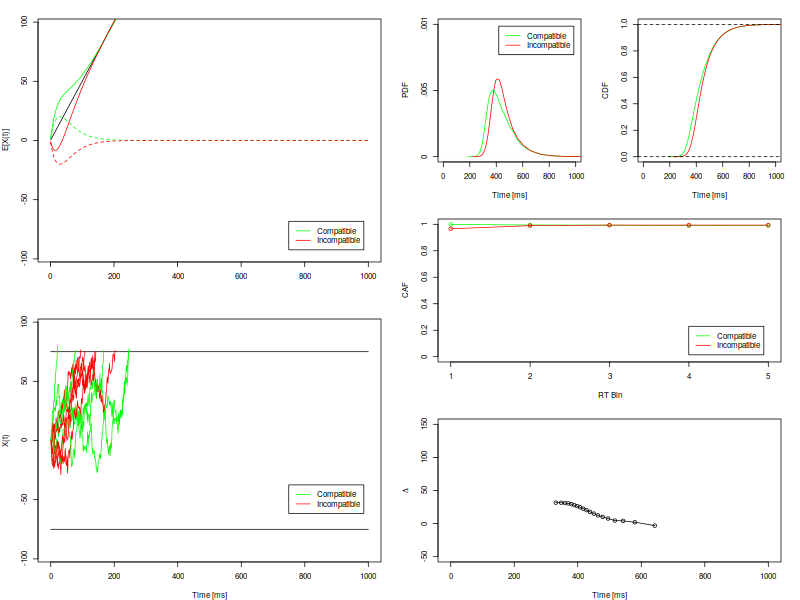
\includegraphics[width=1\textwidth]{../figures/figure1.png}
    \caption{
        DMC simulation. This simulation involved 100,000 trials for each
        compatibility condition with the following default simulation
        parameters: amp = 20, tau = 30, mu = 0.5, bnds = 75, resMean = 300,
        resSD = 30, aaShape = 2. The upper-left panel shows the mean activation
        functions with the black line representing controlled activation. The
        dotted green and red lines represent the automatic activation for
        compatible and incompatible trials, respectively. The solid green and
        red lines represent the sum of controlled and compatible and
        incompatible automatic activation, respectively. The bottom left panels
        shows 5 individual compatible and incompatible trials. A response is
        generated when activation exceeds the boundary level (horizontal
        straight lines). The right upper two panels show the probability
        distribution function (PDF) and the cumulative distribution function
        (CDF) for both compatible and incompatible trials. The middle right
        panel show the conditional accuracy function (CAF) for compatible and
        incompatible trials. The bottom right panel show the delta function for
        the compatibility effect (incompatible - compatible).
    }
    \label{fig:1}
\end{figure}
\textcite{ulrich2015automatic} collected data from both a flanker task and a
simon task and fitted this data to DMC. Here, the delta (RT) and CAF (accuracy)
values from the observed and predicted data were calculated. The model was
fitted by minimising the root-mean-square error (RMSE) weighted difference
between the predicted and observed delta and CAF values using the SIMPLEX
minimization routine of \textcite{nelder1965simplex}.

\section{R Package: DMCfun} 
The R-package DMCfun provides functionality allowing both the simulation of the
DMC model and fitting the model to observed data. The simulation code is
written in C++ utilising the R-package Rcpp \parencite{eddelbuettel2011rcpp}.
The use of C++ gives a significant performance boost over base R whilst the
Rcpp interface allows \DIFdelbegin \DIFdel{convienient }\DIFdelend \DIFaddbegin \DIFadd{convenient }\DIFaddend use from within the standard R environment
and also direct access to plotting facilities within R. The fitting procedure
uses the R-package optimr \textcite{optimr} with method = "Nelder-Mead". As in
\textcite{ulrich2015automatic} the model fit was evaluated by calculating the
RMSE weighted difference between the predicted and observed delta/CAF values.
The following sections will provide a tutorial-type overview of using the
package, both for running the basic simulation and also fitting the observed
data from \textcite{ulrich2015automatic}.

\label{dmc_fun}
\subsection{Gettting Started}
\label{getting_started}
The package is currently hosted on GitHub (https://github.com/igmmgi/DMCfun).
It is anticipated that the package will also be submitted to the R CRAN
repository. The package can be installed directly from GitHub using the
devtools package (via install\_github, see Code Example 1).

\begin{minipage}{\linewidth}
    \begin{lstlisting}[style = R, title={R Code Example 1: instalation}, captionpos=t]
    > # install.packages("devtools")
    > devtools::install_github("igmmgi/DMCfun")
    > library(DMCfun)
    > help(package = "DMCfun")  
    
\end{lstlisting}
\end{minipage}

\subsection{DMC Simulation}
\label{dmc_simulation}
The simulation code is within the functions dmcSim (see Code Example 2).  The
function dmcSim() allows the user to specify parameter values using named
arguments (?dmcSim). A single simulation run with 100,000 trials in each
compatibility condition takes approximately < 150 ms (standard desktop PC).
The function dmcSims allows the user to specify a list of input parameters in
order to run multiple simulations. For example, \textcite{ulrich2015automatic}
observed that the parameter tau ($\tau$) largely determined the slope to the
delta function. In Code Example 3, the DMC simulation is run using tau starting
parameters from 20 to 170 in steps of 10 (see Figure \ref{fig:2}).

\begin{minipage}{\linewidth}
    \begin{lstlisting}[style = R, title = {R Code Example 2}, captionpos = t]
> dmc <- dmcSim(fullData = TRUE)            # Fig 3 from Ulrich et al. (2015)
> dmc <- dmcSim(fullData = TRUE, tau = 150) # Fig 4 from Ulrich et al. (2015)
> plot(dmc)
> plot(dmc, figType = "caf")    
> plot(dmc, figType = "delta")
> 
> dmc <- dmcSim() 
> plot(dmc)       # Fig 3 from Ulrich et al. 

    
\end{lstlisting}
\end{minipage}

\begin{figure}
    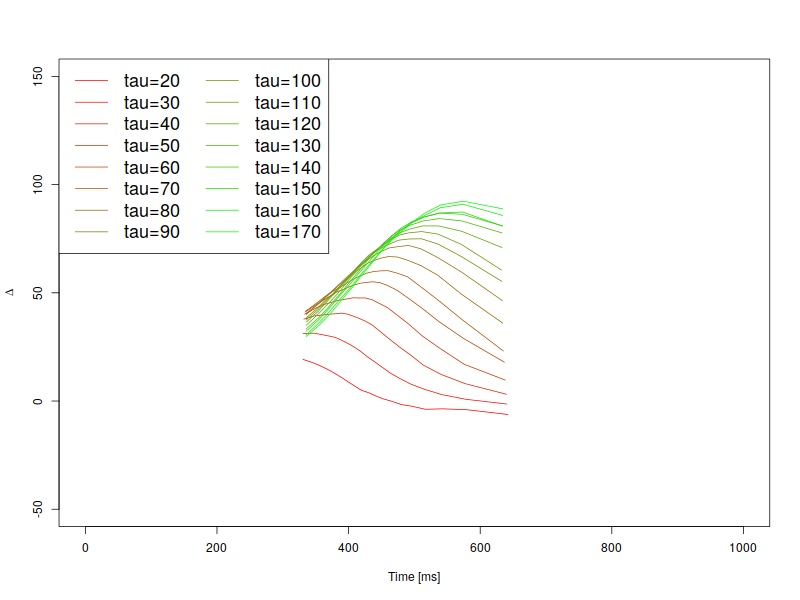
\includegraphics[width=1\textwidth]{../figures/figure4.png}
    \caption{DMC Simulation delta functions with varying tau parameter only.}
    \label{fig:2}
\end{figure}

\subsection{DMC Fit: Real data} 
\label{dmc_fit} 

The package includes the raw data from \textcite{ulrich2015automatic} (see Code
Example 4). This data can be fitted to DMC via the function dmcFitAgg (see Code
Example 5). This will fit DMC to the data averaged across all participants,
whereas the function dmcFitVPs will fit DMC to individual participants. A
summary of the fit is provided. By default, dmcFit* fits the following
parameters: amp, tau, mu, bnds, resMean, resSD, aaShape, spShape. The function
dmcFit* uses the R-package optimr \DIFdelbegin \DIFdel{\textcite{optimr} }\DIFdelend \DIFaddbegin \parencite{optimr} \DIFaddend with method = "Nelder-Mead"
and allow the specification of a number of options including which parameters
to fit and their starting values. \textcite{ulrich2015automatic} observed that
model fit was highly influenced by the tau parameter. The function dmcFit*
first searches a grid space (N = 10) within this single parameter to find the
"best" starting value of tau before the simplex minimisation routine is
implemented. An initial search of a parameter space has been shown to improve
parameter recovery \parencite{hubnerimproving}. Such a initial search grid and
subsequent fitting procedure takes < 1 minute. It is also possible to search
the initial grid space across multiple parameters with the search space being
determined by the input arguments minVals, maxVals, and fitInitialGridN. It
should be noted that increasing the size of the initial grid space will
increase computational time prior to the simplex minimisation routine
dramatically. For example, searching 6 parameters within a gridspace of 6,
results in 46,656 initial parameter sets. Although these are independent and
are run in parallel, such an initial grid space takes approximately 20 minutes
(tested on 12 core desktop PC). As a result, the default setting is to perform
the initial search in the tau space only. Such a procedure produced consistently
good fits with the data of \textcite{ulrich2015automatic} (RMSE < 15), although
this does not exclude the possibility that other datasets would benefit from an
extended search grid (or alternative starting values) regarding the initial
values for the simplex routine.

\begin{minipage}{\linewidth}
    \begin{lstlisting}[style = R, title = {R Code Example 3}, captionpos = t]
> dmc <- dmcSims(list(tau = seq(20,170,10)))
> plot(dmc[[1]])  # full plot first combination
> plot(dmc)       # plot delta functions for each combination
    
\end{lstlisting}
\end{minipage}

Users can fit DMC to their own data using the function dmcObservedData (see
Code Example 6). This function takes an R dataframe (or a *.txt file with tab
separated values, one header line) (see Table 1) and calculates the required
variables. Four data columns are required: one for participant number, one for
compatibility, one for reaction time, and one for error rate. The specific
column names and column codings can be specified using function arguments.

\begin{minipage}{\linewidth}
    \begin{lstlisting}[style = R, title = {R Code Example 4}, captionpos = t]
    flankerDataRaw      # raw flanker data
    flankerData         # summarised flanker data
    flankerData$summary # aggregated flanker data
    plot(flankerData)
    simonDataRaw        # raw simon data
    simonData           # summarised simon data
    simonData$summary   # aggregated simon data
    plot(simonData)
    
\end{lstlisting}
\end{minipage}

\begin{minipage}{\linewidth}
    \begin{lstlisting}[style = R, title = {R Code Example 5}, captionpos = t]
> fit<-dmcFitAgg(flankerData) # flanker data from Ulrich et al. (2015)
> plot(fit,flankerData)
> summary(fit)

# output values from flanker data
# A tibble: 1 x 9 
    amp   tau    mu  bnds resMean resSD aaShape spShape  rmse
  <dbl> <dbl> <dbl> <dbl>   <dbl> <dbl>   <dbl>   <dbl> <dbl>
1  17.7  106. 0.599  55.7    326.  28.8    2.02    3.04  7.50

> fit<-dmcFitAgg(simonData) # simon data from Ulrich et al. (2015)
> plot(fit,simonData)
> summary(fit)

# output values from simon data
# A tibble: 1 x 9
    amp   tau    mu  bnds resMean resSD aaShape spShape  rmse
  <dbl> <dbl> <dbl> <dbl>   <dbl> <dbl>   <dbl>   <dbl> <dbl>
1  17.9  27.9 0.595  58.1    315.  31.5    2.32    3.20  11.6
    
\end{lstlisting}
\end{minipage}



\begin{minipage}{\linewidth}
    \begin{lstlisting}[style = R, title = {R Code Example 6}, captionpos = t]
> ?dmcObservedData
> datOb <- dmcObservedData(datframe, 
                           columns = c("SNo","comp","rt","err"), 
                           compCoding = c(1, 2), 
                           errorCoding = c(0, 1)) 
> plot(datOb)
> dmcFit <- dmcFitAgg(datOb)
> plot(dmcFit,datOb)
    
\end{lstlisting}
\end{minipage}

% latex table generated in R 3.6.1 by xtable 1.8-4 package
%DIF <  Thu Mar  5 09:50:14 2020
%DIF >  Sat Apr  4 12:43:11 2020
\begin{longtable}{rlrr}
\caption{Raw Data file example} \\ 
  \hline
VP & Comp & RT & Error \\ 
  \hline
   1 & comp & 601.657 &    0 \\ 
     1 & comp & 451.429 &    0 \\ 
     1 & comp & 418.097 &    0 \\ 
     1 & incomp & 451.436 &    0 \\ 
     1 & comp & 401.312 &    0 \\ 
     1 & incomp & 434.749 &    0 \\ 
   \hline
\hline
\end{longtable}


\begin{figure}[H]
    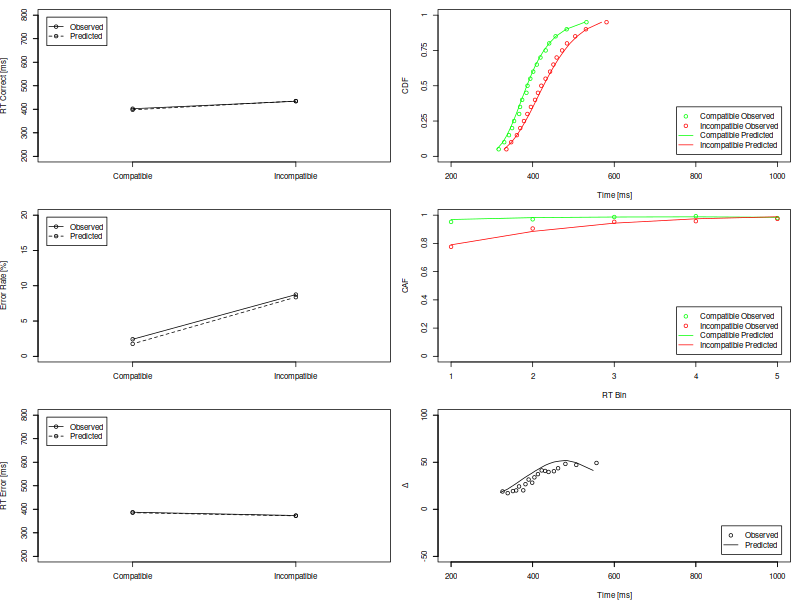
\includegraphics[width=1\textwidth]{../figures/figure5.png}
    \caption{DMC Fit from the Flanker data presented in \textcite{ulrich2015automatic}. Refer to Code Example 5.}
    \label{fig:5}
\end{figure}

\begin{figure}[H]
    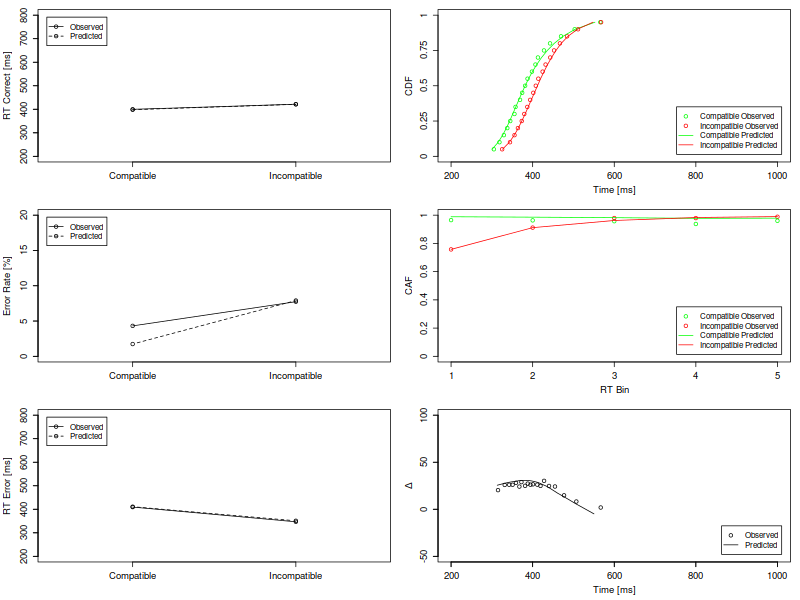
\includegraphics[width=1\textwidth]{../figures/figure6.png}
    \caption{DMC Fit from the Simon data presented in \textcite{ulrich2015automatic}. Refer to Code Example 5.}
    \label{fig:6}
\end{figure}

\section{Conclusions}
\label{summary}
To summarize, the R-package DMCfun provides users with an easy-to-use interface
for both simulating the DMC model with various input parameters and fitting
this model to observed behavioural data from within conflict-like tasks. 

\begin{acknowledgements}
    We would like to thank Rolf Ulrich for providing the raw data from
    \textcite{ulrich2015automatic} and Rolf Ulrich, Hartmut Leuthold, and Victor
    Mittelstädt for providing valuable comments on an earlier draft of this
    manuscript.
\end{acknowledgements}

\section*{Conflict of interest}
The authors declare that they have no conflict of interest.

\section*{The code and data used are available at https://github.com/igmmgi/DMCfun}

\printbibliography
\end{document}
